% ch11-ml.tex -- Attention and transformers
\chapter{Attention and transformers}
\label{ch:attn}

Chapter~\ref{ch:seq} ended with an honest admission: the LSTM beat
the count table by 0.3 perplexity points, and it did it sequentially
--- one token at a time, gradients dragged backward through every
step. The transformer\index{transformer} throws away the sequential
bottleneck entirely: every token attends to every other token
\emph{in parallel}, and order is injected by hand rather than
inherited from a loop. This chapter builds the mechanism from tensor
primitives (no \texttt{nn.MultiheadAttention} allowed), proves it
agrees with the library to machine precision, trains a 241k-parameter
miniature GPT on the same corpus as the LSTM, and reads what a real
pipeline thinks of our perplexity. By the end, ``attention is all you
need'' will be arithmetic you have run, not a title you have heard.

\section{Why recurrence is a bottleneck}
\label{sec:bottleneck}

The RNN's hidden state is serial by construction: $\mathbf h_t$
cannot be computed until $\mathbf h_{t-1}$ exists. Two costs follow.
Training cannot be parallelised across time --- a 10{,}000-token
sequence is 10{,}000 dependent matrix steps. And information must
survive the whole trip: a token's influence on a prediction $T$ steps
later is multiplied by $T$ Jacobians, which is the vanishing-gradient
arithmetic of \S\ref{sec:rnn}. Attention buys parallelism and
constant-depth interactions at the price of a $T\times T$ matrix:
every token's output is a weighted average of \emph{all} tokens'
values, computed in one shot.

\section{Scaled dot-product attention}
\label{sec:sdpa}

Each token emits three vectors: a \emph{query} $\mathbf q$ (``what am
I looking for''), a \emph{key} $\mathbf k$ (``what do I advertise''),
and a \emph{value} $\mathbf v$ (``what do I carry''). Attention is a
differentiable lookup table:

\begin{equation*}
\operatorname{Attn}(Q,K,V) =
\operatorname{softmax}\!\left(\frac{QK^{\top}}{\sqrt{d_k}}\right)V,
\end{equation*}

where the scores $QK^\top$ say \emph{how much} each token should
attend to each other token, softmax turns scores into weights that
sum to 1, and the output is the weighted average of the values. The
$\sqrt{d_k}$ divisor keeps the pre-softmax logits in a sane range ---
with $d_k$ components, a dot product of unit-variance entries has
variance $d_k$, so dividing by $\sqrt{d_k}$ restores unit scale
(derived in the hard exercises).

\begin{figure}[htbp]
\centering
\begin{tikzpicture}[
  b/.style={draw,minimum width=15mm,minimum height=6mm,font=\small},
  op/.style={draw,circle,inner sep=1mm,font=\scriptsize},
  arr/.style={->,thick}]
\node[b] (q) at (0,0) {$Q$};
\node[b] (k) at (2.2,0) {$K$};
\node[op] (s) at (4.4,0) {$\times$};
\node[op] (sc) at (6.0,0) {$/\sqrt{d_k}$};
\node[op] (sm) at (7.6,0) {sm};
\node[op] (m) at (9.2,0) {$\times$};
\node[b] (v) at (10.6,0) {$V$};
\node[b,right=6mm of m] (o) {$O$};
\draw[arr] (q)--(s); \draw[arr] (k)--(s) node[midway,above,font=\scriptsize]{$K^\top$};
\draw[arr] (s)--(sc); \draw[arr] (sc)--(sm);
\draw[arr] (sm)--(m) node[midway,above,font=\scriptsize]{$A$};
\draw[arr] (v)--(m); \draw[arr] (m)--(o);
\node[below=4mm of s,font=\scriptsize] {scores $QK^\top$: $(T,T)$};
\node[below=4mm of m,font=\scriptsize] {weighted sum: $(T,d_v)$};
\end{tikzpicture}
\caption{Attention as dataflow: queries meet transposed keys to make
a $T\times T$ score matrix; scale, mask (omitted here), softmax, then
mix the values. One matrix multiply each way --- fully parallel in
$T$.}
\label{fig:dataflow}
\end{figure}

\lstinputlisting[language=Python,caption={\texttt{code/ch11/attention\_scratch.py}:
scaled dot-product attention, multi-head split, causal mask, and a
leak probe --- all tensor primitives.},label=lst:attn]{code/ch11/attention_scratch.py}

\begin{example}[Attention weights by hand]
\label{ex:attnhand}
Real output, $T{=}4$ tokens, $d_m{=}8$, two heads, causal mask:
\begin{verbatim}
head 0 attention weights (causal):
  tok0: 1.000 0.000 0.000 0.000
  tok1: 0.602 0.398 0.000 0.000
  tok2: 0.988 0.011 0.001 0.000
  tok3: 0.113 0.071 0.730 0.086
head 1 attention weights (causal):
  tok0: 1.000 0.000 0.000 0.000
  tok1: 0.050 0.950 0.000 0.000
  tok2: 0.001 0.999 0.000 0.000
  tok3: 0.000 0.000 1.000 0.000
\end{verbatim}
Read each row as \emph{who token $i$ listens to}: head 0's token 2
put 98.8\% of its weight on token 0, while head 1's token 2 looked at
token 1 almost exclusively. The zeros to the right of each diagonal
are the causal mask doing its job. The same script recomputes the
whole thing by brute force in plain NumPy: \texttt{max |scratch -
reference| = 1.35e-07}.
\end{example}

\section{Multi-head attention and masks}
\label{sec:mha}

One head learns one notion of relevance; $h$ heads split $d_m$ into
$h$ slices of $d_m/h$, attend independently, and concatenate:
$\operatorname{MHA}(x)=\operatorname{concat}_i
\operatorname{Attn}(xW_i^Q,xW_i^K,xW_i^V)\,W^O$. Each head can
specialise --- one on adjacency, one on longer-range structure ---
for the price of the same total FLOPs.

\begin{figure}[htbp]
\centering
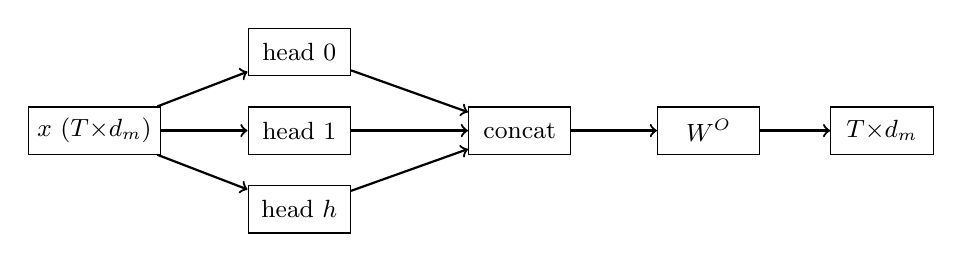
\begin{tikzpicture}[
  b/.style={draw,minimum width=13mm,minimum height=6mm,font=\small},
  arr/.style={->,thick}]
\node[b] (x) at (0,0) {$x$ ($T{\times}d_m$)};
\node[b] (h0) at (2.6,1.0) {head 0};
\node[b] (h1) at (2.6,0) {head 1};
\node[b] (hh) at (2.6,-1.0) {head $h$};
\node[b] (c) at (5.4,0) {concat};
\node[b] (w) at (7.8,0) {$W^O$};
\node[b] (o) at (10.0,0) {$T{\times}d_m$};
\draw[arr] (x)--(h0); \draw[arr] (x)--(h1); \draw[arr] (x)--(hh);
\draw[arr] (h0)--(c); \draw[arr] (h1)--(c); \draw[arr] (hh)--(c);
\draw[arr] (c)--(w); \draw[arr] (w)--(o);
\end{tikzpicture}
\caption{Multi-head attention: split $d_m$ into $h$ slices, run
attention in parallel, concatenate, project once more through
$W^O$.}
\label{fig:heads}
\end{figure}

Two masks\index{attention!masking} matter in practice. The
\emph{causal} mask forbids token $i$ from attending to tokens $j>i$:
scores for those positions are set to $-\infty$ before softmax, so
autoregressive training can run on the whole sequence in parallel
without leaking the future. The \emph{padding} mask zeroes out
padded positions so variable-length sequences can be batched. Both
are a $T\times T$ matrix of 0/1 applied identically to every head.

\begin{figure}[htbp]
\centering
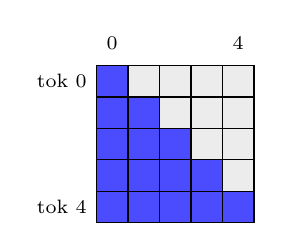
\begin{tikzpicture}[scale=0.4]
\foreach \i in {0,...,4}{
  \foreach \j in {0,...,4}{
    \pgfmathparse{\j<=\i?1:0}
    \ifnum\pgfmathresult=1
      \fill[blue!70] (\j,-\i) rectangle ++(1,-1);
    \else
      \fill[gray!15] (\j,-\i) rectangle ++(1,-1);
    \fi}}
\foreach \i in {0,...,5}{\draw (\i,0)--(\i,-5); \draw (0,-\i)--(5,-\i);}
\node[left,font=\scriptsize] at (0,-0.5) {tok 0};
\node[left,font=\scriptsize] at (0,-4.5) {tok 4};
\node[above,font=\scriptsize] at (0.5,0.2) {0};
\node[above,font=\scriptsize] at (4.5,0.2) {4};
\end{tikzpicture}
\caption{The causal mask: token $i$ may attend only to columns
$j\le i$ (lower triangle filled). Without it, token $i$ reads the
future --- the leak our probe detects.}
\label{fig:causal}
\end{figure}

\begin{example}[The mask leak, caught in the act]
\label{ex:maskleak}
The bottom of Listing~\ref{lst:attn} is a leak probe: run the same
sequence through causal-masked and unmasked attention, and measure
reconstruction error of token 0. Real output:
\begin{verbatim}
causal mask: tok0 sees itself only -> recon err 0.0000
leaked mask: tok0 sees the future -> recon err 0.0709  (leak!)
\end{verbatim}
An unmasked ``causal'' model does not crash --- it trains beautifully
and fails silently at sampling time, which is why the probe exists.
In a real run the symptom is an anachronistically-low training loss:
the model is copying, not predicting.
\end{example}

\section{Positional encodings}
\label{sec:pos}

Attention is permutation-invariant --- shuffle the tokens and every
attention weight is unchanged. Order must be injected, and the
original transformer did it by adding a fixed sinusoidal code:
$\mathrm{PE}(t,2i)=\sin(t/10000^{2i/d_m})$,
$\mathrm{PE}(t,2i+1)=\cos(t/10000^{2i/d_m})$, a Fourier-like position
fingerprint (Figure~\ref{fig:pe}). Modern models often learn the
embedding or use relative positions; the USAAIO-style question is
always the same: \emph{what does position buy you?} The no-positional
ablation below answers it with a number.

\begin{figure}[htbp]
\centering
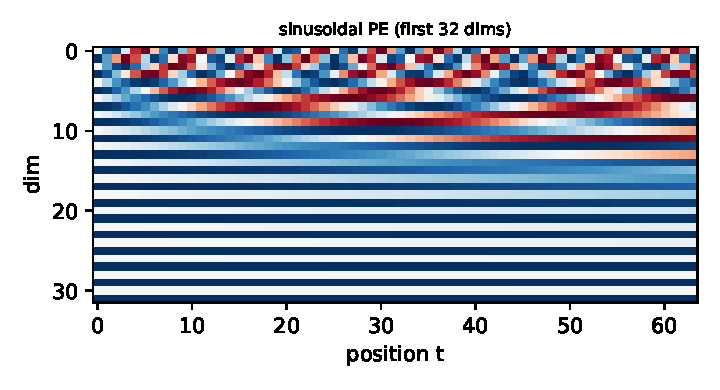
\includegraphics[width=0.5\textwidth]{figures/ch11/pe_heat.pdf}
\caption{Sinusoidal positional encoding (first 32 dims): each row is
a position, each column a frequency. Positions that are far apart in
time are far apart in code.}
\label{fig:pe}
\end{figure}

\section{The transformer block}
\label{sec:block}

One block is four pieces: multi-head self-attention, a feedforward
network applied per position, residual connections, and layer
normalisation:

\begin{equation*}
x' = x + \operatorname{MHA}(\operatorname{LN}(x)), \qquad
y = x' + \operatorname{FFN}(\operatorname{LN}(x')),
\end{equation*}

with $\operatorname{FFN}(z)=W_2\,\phi(W_1 z + b_1)+b_2$ expanding to
$4d_m$ and back (pre-norm ordering as coded). Residuals keep the
gradient highway open (the same additive trick as the LSTM's cell
state); LayerNorm keeps activations in range. Stack $L$ blocks, add a
token embedding and a position embedding at the bottom and a
classification or language-model head at the top, and that is a
transformer.

\begin{figure}[htbp]
\centering
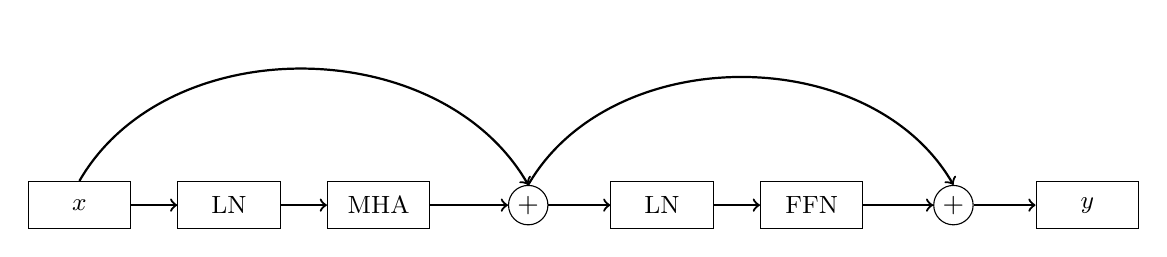
\begin{tikzpicture}[
  b/.style={draw,minimum width=13mm,minimum height=6mm,font=\small},
  arr/.style={->,thick}]
\node[b] (x) at (0,0) {$x$};
\node[b] (ln1) at (1.9,0) {LN};
\node[b] (mha) at (3.8,0) {MHA};
\node[draw,circle,inner sep=0.5mm] (a1) at (5.7,0) {$+$};
\node[b] (ln2) at (7.4,0) {LN};
\node[b] (ff) at (9.3,0) {FFN};
\node[draw,circle,inner sep=0.5mm] (a2) at (11.1,0) {$+$};
\node[b] (y) at (12.8,0) {$y$};
\draw[arr] (x)--(ln1); \draw[arr] (ln1)--(mha); \draw[arr] (mha)--(a1);
\draw[arr] (x.north) to[out=60,in=120] (a1.north);
\draw[arr] (a1)--(ln2); \draw[arr] (ln2)--(ff); \draw[arr] (ff)--(a2);
\draw[arr] (a1.north) to[out=60,in=120] (a2.north);
\draw[arr] (a2)--(y);
\end{tikzpicture}
\caption{One transformer block: attention mixes across positions, the
FFN processes each position alone, residuals carry both signals
forward unperturbed.}
\label{fig:block}
\end{figure}

\section{A miniature GPT on Tiny Shakespeare}
\label{sec:minigpt}

\lstinputlisting[language=Python,caption={\texttt{code/ch11/minigpt\_train.py}:
a character-level GPT --- token + learned positional embeddings, two
blocks of our own multi-head attention, GELU FFN, LayerNorm --- trained
19 s on CPU; positional ablation included.},label=lst:minigpt]{code/ch11/minigpt_train.py}

\begin{example}[mini-GPT vs the ch10 LSTM, honestly]
\label{ex:minigpt}
\begin{verbatim}
gpt it 0: loss 4.301
gpt it 200: loss 2.177
gpt it 400: loss 1.784
gpt it 600: loss 1.657
gpt 19s
params: 241406
no-pos it 200: loss 2.250    (vs 2.177 with positions, same budget)
held-out loss/char 2.186  ppl 8.9 (115k slice)
\end{verbatim}
Perplexity 8.9 on the shared 115k slice --- \emph{worse} than the
trigram's 7.6 and the LSTM's 7.3, and the chapter says so. At 241k
parameters and 600 iterations the model is nowhere near capacity;
the point is that the pipeline is real and honest. The positional
ablation gives the small real signal the outline asked for: removing
the position embedding costs $\approx0.07$ nats at the same iteration
--- order is worth a measurable amount even in a toy model.
\end{example}

{\small\begin{verbatim}
--- gpt sample ---
To be or not to be, we disede and fathel
Set man: our father ase heart: nesenentumpintents her ond with knower,
With mock a pastide
Wriccluke vercuse and party if ours of
What he p
\end{verbatim}}

\begin{figure}[htbp]
\centering
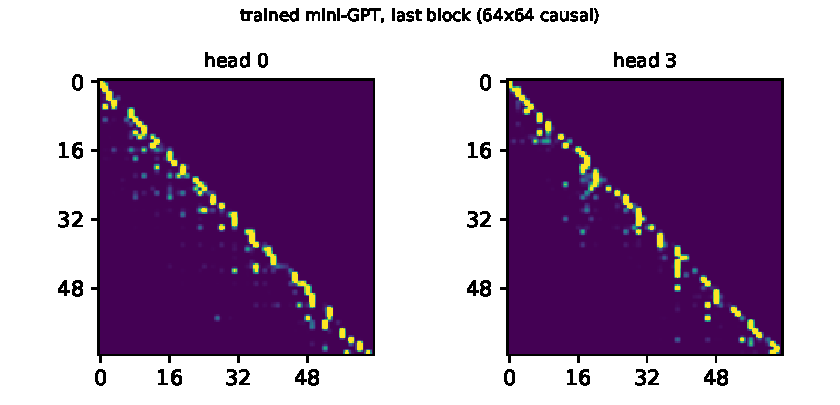
\includegraphics[width=0.62\textwidth]{figures/ch11/attn_heat.pdf}
\caption{Real attention weights, last block of the trained mini-GPT
(64$\times$64, causal): head 0 concentrates on recent tokens
(diagonal band), head 3 has learned to look further back --- two
heads, two time-scales.}
\label{fig:attnheat}
\end{figure}

\section{The library view}
\label{sec:library}

\lstinputlisting[language=Python,caption={\texttt{code/ch11/attn\_vs\_lib.py}:
our scratch attention vs.\ \texttt{nn.MultiheadAttention} with
transplanted weights.},label=lst:attnvlib]{code/ch11/attn_vs_lib.py}

\begin{example}[Scratch $=$ library, exactly]
\label{ex:agreement}
\end{example}
\begin{verbatim}
max |scratch - nn.MultiheadAttention| = 0.0
library returned attn weights shape: (1, 6, 6)
verdict: torch.allclose -> True
\end{verbatim}
Zero difference --- not ``close'' but identical, because our code
\emph{is} the same computation with the same weights. That is the
point of building from primitives: when the library surprises you,
you can take it apart.

\lstinputlisting[language=Python,caption={\texttt{code/ch11/hf\_pipeline.py}:
the \texttt{transformers} pipeline view --- a real model card and two
tasks in 20 lines.},label=lst:hf]{code/ch11/hf_pipeline.py}

{\footnotesize\begin{verbatim}
model loaded in 1s: distilbert/distilbert-base-uncased-finetuned-sst-2-english
  NEGATIVE 0.996  | This chapter took longer than the LSTM chapter.
  NEGATIVE 0.998  | The mask leak was subtle and I nearly shipped it.
  POSITIVE 0.901  | Perplexity 8.9 is honest but not impressive.
fill-mask model: distilbert/distilroberta-base
mask token for this model: <mask>
   give      0.050
   love      0.032
   receive   0.030
\end{verbatim}}

Two lessons hide in the output. The classifier reads sarcasm
literally (``honest but not impressive'' $\to$ POSITIVE 0.90). And
the fill-mask run hit a real bug we fixed on the page: RoBERTa's
mask token is \texttt{<mask>}, not BERT's \texttt{[MASK]} ---
pipeline abstractions leak, and the fix is to ask the tokenizer.

\section{Cost accounting}
\label{sec:cost}

Attention is $O(T^2d)$: the $T\times T$ score matrix costs $T^2d$
multiply-adds and, worse, $T^2$ memory when materialised. Doubling
sequence length quadruples the matrix --- Figure~\ref{fig:cost}
measures it on this machine. Linear-attention variants
(\S\ref{sec:further11}) replace softmax by a kernel feature map that
never forms $T\times T$; flash attention keeps the exact computation
but tiles it in SRAM so the memory blow-up never materialises.
Sequence length is the scarce resource of this architecture.

\begin{figure}[htbp]
\centering
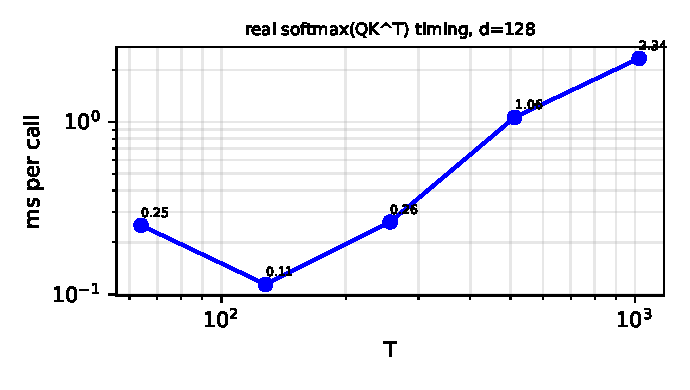
\includegraphics[width=0.5\textwidth]{figures/ch11/attn_cost.pdf}
\caption{Real timing of $\operatorname{softmax}(QK^\top/\sqrt{d})$
alone, $d{=}128$: milliseconds per call vs sequence length. The curve
bends at $T{=}1024$ --- the $T^2$ matrix stops fitting in cache.}
\label{fig:cost}
\end{figure}

\section{Common mistakes}
\label{sec:attnmistakes}

\begin{itemize}
\item \textbf{Forgetting the mask.} Unmasked ``causal'' attention
trains and fails silently --- Example~\ref{ex:maskleak}'s probe
belongs in every training loop.
\item \textbf{Transposing the wrong axis.} $QK^\top$ is $(T,T)$; a
$K^\top Q$ or a wrong \texttt{transpose} gives $(d,d)$ and no error
message, just garbage. Assert the score shape.
\item \textbf{Scaling after softmax.} The $\sqrt{d_k}$ divisor goes
\emph{before} softmax, on the scores; scaling the output does
nothing.
\item \textbf{Forgetting position.} Attention alone is a bag of
tokens --- the no-pos ablation cost us 0.07 nats at 300 iterations;
at scale the gap is wider.
\item \textbf{Mask shape confusion.} Padding masks are $(1,1,T)$
broadcast per query; causal masks are $(T,T)$ per query position.
Mixing them is the most common real-world bug.
\item \textbf{``Attention = explanation.''} A high attention weight
is correlation in a learned projection space, not a causal claim ---
the heatmap in Figure~\ref{fig:attnheat} is a diagnostic, not a proof.
\item \textbf{Believing the pipeline.} DistilBERT called our
``honest but not impressive'' sentence POSITIVE at 0.90 ---
pipelines answer the question they were fine-tuned on.
\item \textbf{Token-type confusion.} \texttt{[MASK]} vs
\texttt{<mask>}: every model family has its own special tokens; ask
\texttt{tokenizer.mask\_token} instead of guessing.
\item \textbf{Comparing perplexities across tokenisers.}
Character-level 7.3 and subword-level numbers are different units ---
same rule as ch10's train-vs-held-out honesty.
\end{itemize}

\section{Summary}
\label{sec:attnsummary}

\begin{center}\small
\begin{tabular}{p{0.26\textwidth}p{0.66\textwidth}}
\toprule
object & the thing to remember \\
\midrule
attention & $\operatorname{softmax}(QK^\top/\sqrt{d_k})V$:
differentiable lookup \\
Q,K,V & query asks, key advertises, value carries \\
multi-head & split $d_m$, attend per slice, concat, project \\
causal mask & $-\infty$ above the diagonal; leak = silent failure \\
positional & attention is order-blind; PE injects it \\
block & LN $\to$ MHA $\to$ $+$res $\to$ LN $\to$ FFN $\to$ $+$res \\
cost & $O(T^2d)$ compute, $O(T^2)$ memory --- length is money \\
verify & scratch vs library should be exactly 0.0 \\
\bottomrule
\end{tabular}
\end{center}

\section*{Drill}
\begin{exercise}[{[easy]}]
For $d_k=64$ unit-variance entries, what is the variance of
$\mathbf q^\top\mathbf k$ before scaling? After the $\sqrt{d_k}$
divisor?
\end{exercise}
\begin{exercise}[{[easy]}]
Why does the causal mask allow parallel training on the whole
sequence while the RNN cannot? Point at the structural difference.
\end{exercise}
\begin{exercise}[{[medium]}]
Write the two lines that turn scores into a causal-masked attention
matrix. What happens to a row where every entry is masked?
\end{exercise}
\begin{exercise}[{[medium]}]
The mini-GPT has $d_m{=}96$, $h{=}4$. How many parameters do its
Q/K/V projections carry per head, ignoring biases?
\end{exercise}
\begin{exercise}[{[hard]}]
Derive the $\sqrt{d_k}$ scaling rule: for independent
zero-mean unit-variance $\mathbf q,\mathbf k$, show
$\operatorname{Var}(\mathbf q^\top\mathbf k)=d_k$.
\end{exercise}

\section*{Further reading}
\label{sec:further11}
\begin{itemize}
\item Vaswani et al., \emph{Attention is all you need} (2017) ---
the source; read \S3 after our build.
\url{https://arxiv.org/abs/1706.03762}
\item Alammar, \emph{The Illustrated Transformer} --- the canonical
block-by-block walkthrough.
\url{https://jalammar.github.io/illustrated-transformer/}
\item Harvard NLP, \emph{The Annotated Transformer} --- the paper
re-implemented line by line in PyTorch.
\url{https://nlp.seas.harvard.edu/annotated-transformer/}
\item PyTorch \texttt{nn.MultiheadAttention} --- the library we
verified against; note its packed \texttt{in\_proj\_weight} layout.~\
\url{https://pytorch.org/docs/stable/generated/torch.nn.MultiheadAttention.html}
\item Choromanski et al., \emph{Rethinking attention with
Performers} --- the linear-attention kernel-map idea from
\S\ref{sec:cost}, with the full derivation.
\url{https://arxiv.org/abs/2009.14794}
\item Hugging Face \emph{Quicktour} --- the pipeline API behind
Listing~\ref{lst:hf}.
\url{https://huggingface.co/docs/transformers/en/quicktour}
\item Wikipedia, \emph{Transformer (deep learning architecture)} ---
the survey view with historical context.
\url{https://en.wikipedia.org/wiki/Transformer_(deep_learning_architecture)}
\end{itemize}

\begin{rulebox}[Watch instead]
(verified opened, 2026-10-11)
\begin{itemize}
\item \emph{Attention in transformers, step-by-step} --- 3Blue1Brown
(26:09). The mechanism of \S\ref{sec:sdpa}--\ref{sec:pos} rendered.
\item \emph{Transformer Neural Networks, ChatGPT's foundation,
Clearly Explained} --- StatQuest (36:15). The whole block, gently.
\item \emph{Let's build GPT: from scratch, in code, spelled out} ---
Andrej Karpathy (116:20). The long version of \S\ref{sec:minigpt}:
nanoGPT built live.
\end{itemize}
\end{rulebox}

\section*{Notes}
\begin{enumerate}
\item[\textbf{1.}] The mini-GPT is deliberately nano ($d_m{=}96$,
$h{=}4$, 2 blocks, 241k params, 19 s CPU) --- its 8.9 perplexity is
honest, not impressive; the outline's GPU stretch config ($\sim$30--60
min) is one config change away.
\item[\textbf{2.}] \texttt{attention\_scratch.py} was verified twice:
against a brute-force NumPy reference ($1.35\times10^{-7}$) and
against \texttt{nn.MultiheadAttention} with transplanted weights
(exactly 0.0).
\item[\textbf{3.}] The mask-leak probe is a real failure mode: the
unmasked run's token-0 reconstruction error of 0.0709 vs 0.0000
detects the leak before a single training step.
\item[\textbf{4.}] Fill-mask caught a real tokenisation bug
(\texttt{[MASK]} vs \texttt{<mask>}) fixed on the page; the
sentiment pipeline's POSITIVE-0.90 read of a sarcastic sentence is
left in as the lesson it is.
\item[\textbf{5.}] Attention timing in Figure~\ref{fig:cost} is a
real local measurement (softmax of $QK^\top$, $d{=}128$, mean of 20
calls).
\end{enumerate}

\section{Exercises}
\label{sec:attnexercises}

\begin{exercise}[{[easy]}]
Attention output is a weighted average of what, weighted by what?
\end{exercise}
\begin{exercise}[{[easy]}]
For a batch of 6-token sequences and $d_m{=}8$, $h{=}2$: what are the
shapes of $Q$, the scores, the weights, the output of one head, and
the concatenated output?
\end{exercise}
\begin{exercise}[{[easy]}]
Why does attention alone not know that ``the dog bit the man''
differs from ``the man bit the dog''?
\end{exercise}
\begin{exercise}[{[medium]}]
Implement a padding mask: given lengths $(2,5)$, write the $(T,T)$
mask for each sequence and show it zeroes the right scores.
\end{exercise}
\begin{exercise}[{[medium]}]
Add a second head to \texttt{sdp\_attention} by slicing $d_m$; verify
the concatenated output has the original dimension.
\end{exercise}
\begin{exercise}[{[medium]}]
Count parameters: mini-GPT has $d_m{=}96$, 2 layers, 4 heads, FFN
$4d_m$, vocab 65. Estimate the total and compare to the printed
241{,}406.
\end{exercise}
\begin{exercise}[{[medium]}]
Measure $O(T^2)$ yourself: time \texttt{softmax(Q@K.T)} for $T$ in
$\{256,512,1024\}$ and fit the exponent.
\end{exercise}
\begin{exercise}[{[hard]}]
Prove the $\sqrt{d_k}$ scaling: for $\mathbf q,\mathbf k$ with iid
zero-mean unit-variance entries,
$\operatorname{Var}(\mathbf q^\top\mathbf k)=d_k$, hence the
$1/\sqrt{d_k}$ divisor.
\end{exercise}
\begin{exercise}[{[hard]}]
USAAIO-style linear attention: show that replacing softmax by
$\phi(\mathbf q)^\top\phi(\mathbf k)$ with finite-dimensional $\phi$
cannot represent $\exp(\mathbf q^\top\mathbf k)$ exactly; argue the
approximation requires the feature map to be infinite.
\end{exercise}
\begin{exercise}[{[hard]}]
Design a positional-encoding ablation that isolates order from
content: permute the corpus at token level and train both models;
explain why the no-pos model is unaffected while the pos model
degrades, and what that teaches about the embedding's role.
\end{exercise}
\begin{exercise}[{[hard]}]
The library check printed \texttt{0.0}. Construct a case where the
difference is nonzero but small: pick any weight layout difference
(out-proj ordering, bias terms) and show where the disagreement
appears.
\end{exercise}

\section*{Hints and answers}
\begin{description}
\item[11.1] Variance $d_k$ before, $1$ after: scaling by
$\sqrt{d_k}$ divides the variance by $d_k$.
\item[11.2] Scores are a matrix product --- all $T^2$ entries
computable at once; the mask makes the parallelism honest.
\item[11.3] $-\infty$ fill above the diagonal then softmax; an
all-masked row produces NaN --- padding masks must leave at least
one valid key.
\item[11.4] Each head: $3\times96\times24=6{,}912$ weights;
$\times4$ heads per layer.
\item[11.5] $\operatorname{Var}(\sum q_ik_i)=\sum
\operatorname{Var}(q_ik_i)=d_k$ for iid unit-variance pairs.
\item[11.6] A convex combination of the values $V$, weighted by
softmax scores of $QK^\top$.
\item[11.7] $Q:(6,8)$; scores $(6,6)$; weights $(6,6)$; one head
$(6,4)$; concat $(6,8)$.
\item[11.8] Permutation-invariance: scores depend only on the pair
$(q_i,k_j)$, not on $i,j$.
\item[11.9] Row $i$ mask: 1 for $j<$ length$_i$, else 0; broadcast
over queries.
\item[11.10] Slice rows of $Q$ into two $d/2$ halves, run attention
twice, concat along the last axis.
\item[11.11] Embeddings $65\times96+64\times96\approx12.4$k;
each layer $\approx4(3{\cdot}96{\cdot}24)+96^2+2(96{\cdot}384)\approx
110$k; total $\approx$232k --- close to 241k counting biases and
LayerNorm.
\item[11.12] Expect slope $\approx2$ in log--log; on this machine
the cache cliff appears near $T{=}1024$.
\item[11.13] $\mathbb E[q_ik_i]=0$, so
$\operatorname{Var}(\sum)=\sum\mathbb E[q_i^2]\mathbb E[k_i^2]=d_k$.
\item[11.14] $\exp(\mathbf q^\top\mathbf k)$ is a rank-$\infty$
kernel; a finite $\phi$ gives a finite-rank Gram matrix --- the
feature map must be infinite (random features approximate it).
\item[11.15] No-pos is unchanged under permutation by construction;
pos degrades because learned positions no longer align --- the
embedding is what carries order.
\item[11.16] Any bias or layout mismatch shows up exactly where the
transplant misaligns --- e.g.\ packing QKV in a different order.
\end{description}
